% =====================================================================
%  NOTE DE SYNTHÈSE — Se loger en France, 2006-2025 (4 pages)
%  Compilation : xelatex note_logement_2026.tex (x2)
%  Chiffres : sorties de l'étude SRCV après correction du niveau de vie
%  (30 septembre 2026) — scripts 09, 12, 19, 23, 29, 30.
% =====================================================================
\documentclass[11pt,a4paper]{article}

\usepackage{fontspec}
\setmainfont{EB Garamond}
\newfontfamily\headingfont{EB Garamond}

\usepackage[a4paper,top=2.9cm,bottom=2cm,left=2.4cm,right=2.4cm,headheight=29pt]{geometry}
\usepackage{xcolor}
\definecolor{brandnavy}{HTML}{243443}
\definecolor{brandgrey}{HTML}{595959}
\definecolor{fond}{HTML}{EEF1F4}

\usepackage{graphicx}
\usepackage{titlesec}
\usepackage{fancyhdr}
\usepackage{enumitem}
\usepackage{microtype}
\usepackage{booktabs}
\usepackage{array}
\newcolumntype{C}[1]{>{\centering\arraybackslash}p{#1}}
\usepackage[flushleft]{threeparttable}
\usepackage{float}
\usepackage[hidelinks]{hyperref}

\renewcommand{\tablename}{Tableau}
\renewcommand{\figurename}{Figure}
\usepackage{caption}
\captionsetup{font=small,labelfont={color=brandnavy},textfont={color=brandnavy},labelsep=colon,skip=4pt}

\hyphenpenalty=10000
\exhyphenpenalty=10000
\tolerance=9999
\emergencystretch=3em
\setlength{\parindent}{0pt}
\setlength{\parskip}{0.55em}

\titleformat{\section}{\headingfont\color{brandnavy}\large}{\thesection.}{0.5em}{}
\titlespacing*{\section}{0pt}{1.1em}{0.4em}

\newcommand{\logoPathi}{assets/logo1.jpg}
\pagestyle{fancy}
\fancyhf{}
\renewcommand{\headrulewidth}{0.4pt}
\fancyhead[L]{\footnotesize\color{brandgrey}\itshape Se loger en France, 2006-2025}
\fancyhead[R]{\raisebox{-0.2\height}{\includegraphics[height=0.95cm]{\logoPathi}}}
\fancyfoot[C]{\footnotesize\color{brandgrey}\thepage}

% Valeur non significative au seuil de 5 %
\newcommand{\ns}[1]{\textcolor{brandgrey}{\textit{#1}}}

\begin{document}

% ------------------------------ Titre ---------------------------------
{\headingfont\color{brandnavy}\fontsize{22}{26}\selectfont Se loger en France, 2006-2025}\\[0.25em]
{\headingfont\color{brandnavy}\large\itshape Moins d'espace pour les locataires, et ce que cela change à la natalité}\\[0.3em]
{\small\color{brandgrey} GENNA Kévin \,·\, Septembre 2026}

\vspace{0.4em}
\noindent\colorbox{fond}{\begin{minipage}{\dimexpr\linewidth-2\fboxsep\relax}
\vspace{0.2em}
{\headingfont\color{brandnavy}\large En bref}
\begin{itemize}[leftmargin=1.1em,itemsep=0.25em,topsep=0.3em]
	\item \textbf{Les locataires ont perdu de l'espace, pas du pouvoir d'achat.} Entre 2014 et 2025, les locataires de 20 à 39 ans ont perdu de 1 à 6 m² selon l'âge, alors que leur taux d'effort a légèrement reculé. Les accédants ont gardé leurs surfaces et vu leur taux d'effort baisser de 4 à 8 points.
	\item \textbf{La moyenne est trompeuse.} La surface moyenne des couples en âge d'avoir des enfants n'a pas bougé depuis 2010. Mais la part des ménages logés dans moins de 60 m² a progressé chez les locataires, à tous les âges.
	\item \textbf{Pour la natalité, seule la surface compte, et sous la forme d'un seuil.} Sous 60 m², un couple sans enfant a 6 à 10 points de chances en moins d'avoir un premier enfant, pour une probabilité moyenne de 14,5\,\%. À surface donnée, ni le prix du mètre carré ni le revenu du ménage ne font de différence.
	\item \textbf{Le logement n'explique pas pour autant la baisse de la fécondité.} Même lu comme causal, ce qui est douteux, le canal des petites surfaces ne pèse que 5 à 8\,\% de la baisse depuis 2010, et la progression de l'accession à la propriété l'a plus que compensé.
\end{itemize}
\vspace{0.1em}
\end{minipage}}

{\small\textit{Sources et définitions.} Enquête Statistiques sur les ressources et conditions de vie (SRCV) de l'Insee, huit vagues : 2006, 2010, 2014, 2018, puis chaque année de 2022 à 2025. Trois statuts d'occupation : les locataires, les propriétaires \textit{accédants}, qui remboursent un emprunt, et les propriétaires \textit{non accédants}, qui n'en remboursent plus ou sont logés gratuitement. Le coût du logement comprend les charges et, pour les accédants, la mensualité d'emprunt. Le taux d'effort rapporte ce coût annuel au revenu disponible. Montants en euros constants de 2025.}

% ----------------------------------------------------------------------
\section{Les locataires ont perdu de l'espace, les accédants du taux d'effort}

Depuis 2014, les jeunes locataires se logent plus petit sans payer davantage. Leur taux d'effort a même légèrement reculé, de 1 à 5 points selon l'âge, et reste proche d'un tiers du revenu au-delà de 25 ans. Mais le prix du mètre carré loué a augmenté de 4 à 12\,\% en euros constants : la surface a servi de variable d'ajustement, jusqu'à 6 m² de moins chez les 35-39 ans (tableau \ref{tab:evol}).

Chez les propriétaires accédants, la surface achetée est restée stable, autour de 90 m² avant 30 ans et de 105 m² après, et le taux d'effort a reculé de 4 à 8 points. Ce recul s'est poursuivi malgré la remontée des taux d'intérêt en 2022-2024 : il tient sans doute aussi à la composition des accédants, plus aisés quand le crédit se resserre.

\begin{table}[H]
	\centering
	\small
	\setlength{\tabcolsep}{5pt}
	\begin{threeparttable}
		\caption{Conditions de logement des 20-39 ans, 2014 et 2025}
		\label{tab:evol}
		\begin{tabular}{lcrrcrr}
			\toprule
			& \multicolumn{3}{c}{Locataires} & \multicolumn{3}{c}{Propriétaires accédants} \\
			\cmidrule(lr){2-4} \cmidrule(lr){5-7}
			Âge & Surface (m²) & Coût & Effort & Surface (m²) & Coût & Effort \\
			& 2014 → 2025 & (€/mois) & (points) & 2014 → 2025 & (€/mois) & (points) \\
			\midrule
			20-24 ans & 52,9 → 51,7 & +34 & −1,5 & --- & --- & --- \\
			25-29 ans & 61,6 → 58,4 & −36 & −3,3 & 93,4 → 90,0 & −108 & −5,5 \\
			30-34 ans & 64,5 → 61,1 & +39 & −1,4 & 103,6 → 103,5 & −290 & −8,4 \\
			35-39 ans & 71,5 → 65,4 & −14 & −4,8 & 105,4 → 107,9 & −66 & −4,4 \\
			\bottomrule
		\end{tabular}
		\begin{tablenotes}[flushleft]\scriptsize
			\item \textit{Champ} : ménages dont la personne de référence a 20 à 39 ans, France entière. Coût et effort : écart entre 2014 et 2025.
			\item \textit{Lecture} : entre 2014 et 2025, la surface moyenne des locataires de 35-39 ans est passée de 71,5 à 65,4 m², leur coût mensuel a baissé de 14 € et leur taux d'effort de 4,8 points. --- : moins de 30 observations.
		\end{tablenotes}
	\end{threeparttable}
\end{table}

Deux nuances complètent ce tableau. Sur une période plus longue, de 2006 à 2025, la perte de surface des locataires croît avec le revenu : entre 30 et 39 ans, elle est de 4\,\% dans le quintile de niveau de vie le plus modeste et de 20\,\% dans le plus aisé, où le prix du mètre carré a progressé de 36\,\%. Les locataires aisés ont continué à payer, mais pour moins d'espace. Les locataires se sont aussi concentrés dans les grandes agglomérations. Parmi les ménages locataires comptant une femme de 15 à 49 ans, 23\,\% vivent dans l'agglomération parisienne en 2025, contre 15\,\% en 2014, alors que cette part reste proche de 14\,\% chez les accédants. Une partie de la perte de surface tient donc sans doute à ce déplacement vers les marchés les plus chers, plutôt qu'à des logements plus petits à lieu donné.

% ----------------------------------------------------------------------
\section{La moyenne ne bouge pas, le bas de la distribution s'épaissit}

Sur l'ensemble des couples en âge d'avoir des enfants, ces deux mouvements s'annulent en moyenne. La surface moyenne de leur logement est la même en 2010 et en 2025, 101 m² (tableau \ref{tab:champ}). La part des accédants, mieux logés, a progressé de 47 à 52\,\% pendant que les locataires se serraient. Une moyenne stable peut pourtant cacher une distribution qui se déforme. La médiane a perdu 5 m², et la part des couples sans enfant logés dans moins de 60 m² est passée de 27,6 à 30,6\,\%.

\begin{table}[H]
	\centering
	\small
	\setlength{\tabcolsep}{8pt}
	\begin{threeparttable}
		\caption{Le logement des couples en âge d'avoir des enfants, 2010 et 2025}
		\label{tab:champ}
		\begin{tabular}{lrr}
			\toprule
			& 2010 & 2025 \\
			\midrule
			Surface moyenne du logement (m²) & 101,2 & 100,9 \\
			Surface médiane du logement (m²) & 95 & 90 \\
			Couples sans enfant logés dans moins de 60 m² (\%) & 27,6 & 30,6 \\
			Couples sans enfant logés dans moins de 50 m² (\%) & 15,1 & 19,1 \\
			Coût au m² (€/mois) & 13,29 & 13,94 \\
			Part des locataires (\%) & 38,2 & 37,9 \\
			Part des propriétaires accédants (\%) & 46,8 & 52,1 \\
			Part des propriétaires non accédants (\%) & 15,0 & 10,0 \\
			\bottomrule
		\end{tabular}
		\begin{tablenotes}[flushleft]\scriptsize
			\item \textit{Champ} : ménages en couple dont la femme, personne de référence ou conjointe, a 15 à 49 ans, France entière. « Sans enfant » : aucun enfant ne vit dans le ménage. Coût au m² en euros constants de 2025.
		\end{tablenotes}
	\end{threeparttable}
\end{table}

La figure \ref{fig:sous60} montre où se loge ce glissement. La part des ménages vivant dans moins de 60 m² augmente chez les locataires, et à tous les âges : de 49 à 58\,\% avant 30 ans, de 31 à 43\,\% entre 30 et 39 ans, de 2006 à 2025. Chez les propriétaires, elle reste nettement plus basse. Le phénomène touche aussi les couples locataires sans enfant, ceux chez qui se décide le premier enfant : entre 30 et 39 ans, près de la moitié d'entre eux vivent dans moins de 60 m² en 2025, contre environ un tiers en 2006 --- un ordre de grandeur, ces couples n'étant qu'une centaine par vague.

\begin{figure}[H]
	\centering
	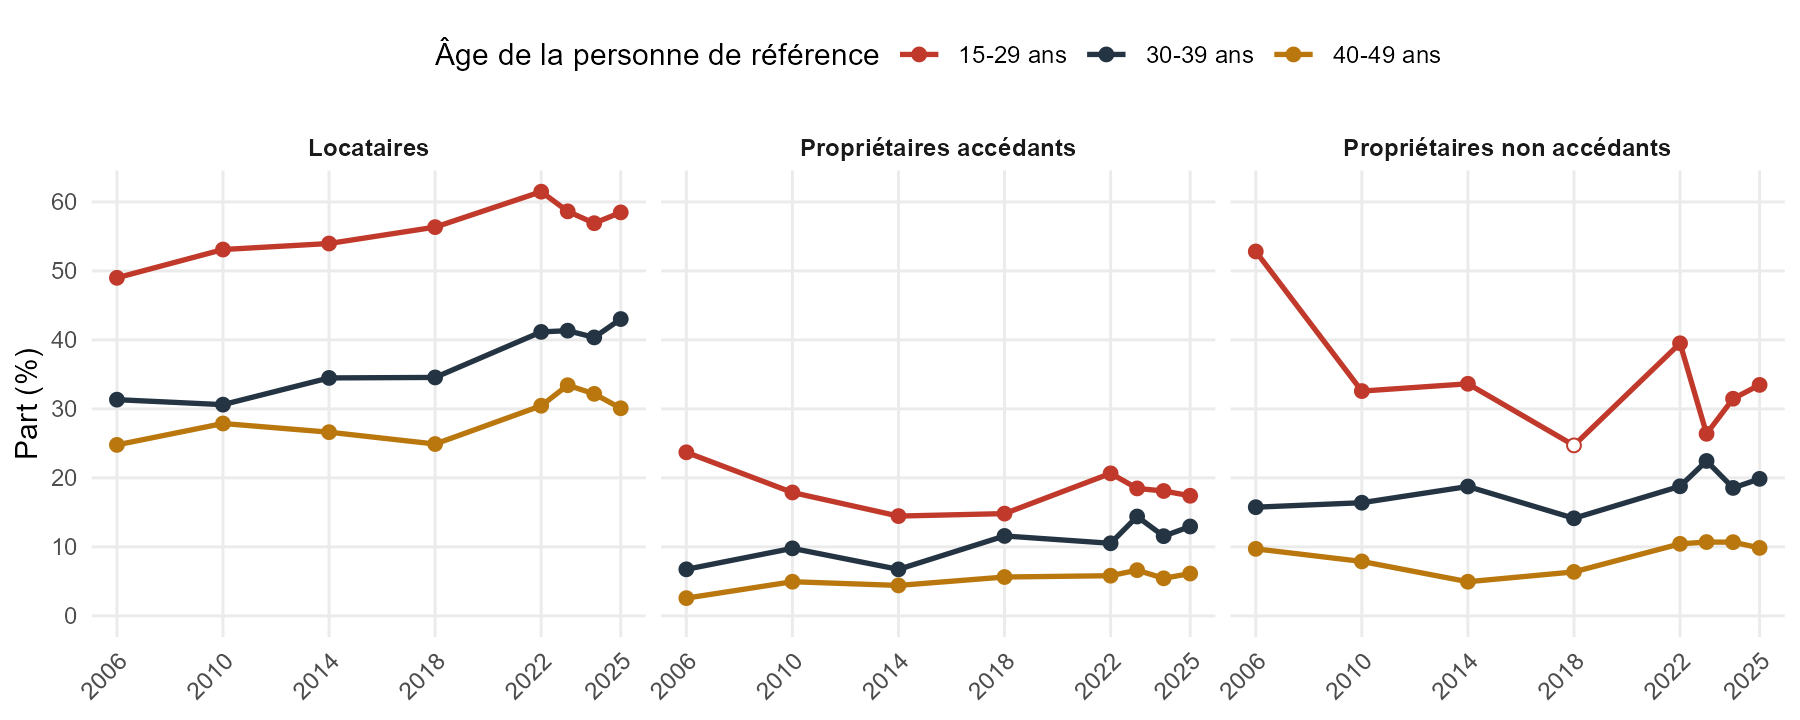
\includegraphics[width=\linewidth]{fig_sous60_tous_menages}
	\caption{Part des ménages logés dans moins de 60 m², selon le statut d'occupation et l'âge de la personne de référence (\%)}
	\label{fig:sous60}
	\par\vspace{0.15em}
	{\scriptsize \textit{Champ} : ménages dont la personne de référence a 15 à 49 ans, en couple ou non, avec ou sans enfant. Points creux : moins de 30 observations. Moyennes pondérées.\par}
\end{figure}

% ----------------------------------------------------------------------
\section{Surface et natalité : une marche, pas une pente}

Pour relier logement et naissances, nous estimons la probabilité qu'un couple déclare une naissance récente. Le champ est celui des couples dont la femme a 15 à 49 ans, soit 26\,470 observations et 2\,118 naissances sur les huit vagues. Le modèle tient compte de l'âge, du revenu, de la catégorie sociale, de la géographie et de l'année. Le revenu y est mesuré avant la naissance et hors prestations familiales, minima sociaux et aides au logement : mesuré après, il baisse mécaniquement avec l'arrivée de l'enfant et fabrique un faux effet négatif du revenu sur la natalité. Quatre résultats en ressortent.

\textbf{Seule la surface compte.} À surface donnée, ni le prix du mètre carré ni le revenu du ménage n'ont d'effet sur la probabilité d'une naissance. Dix mètres carrés de plus sont associés à 0,4 point de probabilité supplémentaire, et à 0,7 point pour un premier enfant. Le débat public raisonne en prix, alors que ce qui compte est ce que le prix permet d'occuper.

\textbf{C'est le premier enfant qui est concerné, et sous la forme d'un seuil.} Chez les couples sans enfant, la probabilité d'une première naissance chute sous 60 m² et ne bouge presque plus au-dessus (tableau \ref{tab:seuil}). La règle n'est donc pas « plus c'est grand, plus on fait d'enfants », mais plutôt « en dessous d'une soixantaine de mètres carrés, on fonde rarement une famille ». Pour les naissances suivantes, l'effet est bien plus faible et le seuil n'est plus significatif.

\begin{table}[H]
	\centering
	\small
	\setlength{\tabcolsep}{7pt}
	\begin{threeparttable}
		\caption{Surface du logement et première naissance}
		\label{tab:seuil}
		\begin{tabular}{lC{3.6cm}C{1.9cm}C{1.9cm}}
			\toprule
			& Écart de probabilité & \multicolumn{2}{c}{Couples sans enfant logés} \\
			& de première naissance & \multicolumn{2}{c}{dans la tranche (\%)} \\
			\cmidrule(lr){3-4}
			Surface du logement & (points) & 2010 & 2025 \\
			\midrule
			Moins de 40 m² & −10,4 & 6,4 & 7,1 \\
			40 à 49 m² & −7,6 & 8,6 & 12,1 \\
			50 à 59 m² & −6,0 & 12,5 & 11,5 \\
			60 à 69 m² & \ns{+2,9} & 16,3 & 14,3 \\
			70 à 89 m² & \textit{réf.} & 24,7 & 21,9 \\
			90 à 119 m² & \ns{+3,5} & 20,2 & 19,7 \\
			120 m² et plus & \ns{+4,1} & 11,3 & 13,5 \\
			\bottomrule
		\end{tabular}
		\begin{tablenotes}[flushleft]\scriptsize
			\item \textit{Champ} : couples sans enfant dont la femme a 15 à 49 ans ; 5\,920 observations, 827 premières naissances. Probabilité moyenne de première naissance : 14,5\,\%.
			\item \textit{Lecture} : à âge, revenu, catégorie sociale, géographie et année donnés, un couple sans enfant logé entre 40 et 49 m² a une probabilité de première naissance inférieure de 7,6 points à celle d'un couple logé entre 70 et 89 m². En gris italique : écart non significatif au seuil de 5\,\%.
		\end{tablenotes}
	\end{threeparttable}
\end{table}

\textbf{Les accédants ont un avantage propre pour le premier enfant.} À âge et revenu égaux, un couple accédant sans enfant a une probabilité de première naissance supérieure d'environ 5 points à celle d'un couple locataire. Un cinquième seulement de cet écart passe par la surface. Pour les naissances suivantes, c'est l'inverse : à caractéristiques égales, les accédants ont une probabilité inférieure de 1,6 point à celle des locataires.

\textbf{L'effet paraît plus fort là où le marché est tendu, sans que ce soit établi.} Dix mètres carrés de plus sont associés à 0,6 point de probabilité de naissance supplémentaire dans l'agglomération parisienne, contre 0,2 point en commune rurale, mais les écarts entre territoires ne sont pas statistiquement significatifs.

\textbf{Une association, probablement pas une causalité.} Ces résultats décrivent une corrélation robuste, pas un effet démontré. Le test le plus exigeant suit les mêmes ménages d'une vague à l'autre. Sur ces ménages, la surface est associée à la naissance qui vient d'avoir lieu (+0,26 point pour 10 m²), mais elle ne prédit pas la naissance suivante (+0,09 point, non significatif). Ce profil ressemble davantage à un logement choisi en fonction d'un projet de famille qu'à une contrainte qui empêcherait ce projet.

% ----------------------------------------------------------------------
\section{Quelle part de la baisse de la fécondité ?}

L'indicateur conjoncturel de fécondité est passé de 2,03 enfants par femme en 2010 à 1,56 en 2025, soit une baisse de 23\,\% (Insee). Pour mesurer ce que le logement peut en porter, nous donnons aux couples de 2025 les conditions de logement de 2010, puis nous recalculons leur probabilité de naissance. Ces conditions sont la distribution des surfaces, le prix au mètre carré et la répartition entre locataires et propriétaires.

\noindent\colorbox{fond}{\begin{minipage}{\dimexpr\linewidth-2\fboxsep\relax}
\small\textbf{Un calcul de coin de table.} La part des couples sans enfant logés sous 60 m² a gagné 3 points entre 2010 et 2025. Chacun de ces couples a environ 9 points de chances en moins d'avoir un premier enfant. Le produit fait 0,3 point sur une probabilité de 14,5\,\%, soit 2\,\% de premières naissances en moins. L'effet est réel, mais il est petit face à une baisse de 23\,\%.
\end{minipage}}

\begin{table}[H]
	\centering
	\small
	\setlength{\tabcolsep}{6pt}
	\begin{threeparttable}
		\caption{Ce que le logement reproduit de la baisse de la fécondité, 2010-2025}
		\label{tab:decompo}
		\begin{tabular}{llr}
			\toprule
			Canal & Évolution 2010-2025 & Part de la baisse (\%) \\
			\midrule
			Petites surfaces & sans enfant sous 60 m² : 27,6 → 30,6\,\% & +5 à +8 \\
			Prix au mètre carré & +4,9\,\% en euros constants & ≈ 0 \\
			Accession à la propriété & accédants : 46,8 → 52,1\,\% & ≈ −10 \\
			\midrule
			\textbf{Logement dans son ensemble} & & \textbf{−7 à −3} \\
			\textit{Sans le canal de l'accession} & & \textit{+4 à +7} \\
			\bottomrule
		\end{tabular}
		\begin{tablenotes}[flushleft]\scriptsize
			\item \textit{Lecture} : si les couples de 2025 avaient connu la distribution des surfaces de 2010, leur probabilité de naissance serait plus élevée d'un montant égal à 5 à 8\,\% de la baisse de l'indicateur conjoncturel de fécondité. Une part négative signifie que l'évolution a joué contre la baisse.
			\item \textit{Fourchettes} : seuil de surface placé à 60 ou à 50 m². Ces parts supposent que l'effet mesuré sur les couples se transpose à l'ensemble des femmes et que le lien entre logement et naissance soit causal : ce sont des ordres de grandeur, et des plafonds. Elles résistent aux fragilités de mesure des vagues récentes.
		\end{tablenotes}
	\end{threeparttable}
\end{table}

Le logement joue donc par deux canaux de sens contraire. La montée des petites surfaces chez les locataires a pesé sur la natalité, pour 5 à 8\,\% de la baisse selon le seuil retenu. La progression de l'accession à la propriété l'a soutenue d'un montant un peu supérieur, si bien que le solde est nul, voire légèrement favorable (tableau \ref{tab:decompo}). L'avantage des accédants peut toutefois refléter des couples qui avaient déjà décidé de s'installer. Si on l'écarte, la part du logement plafonne sous un dixième de la baisse. À titre de comparaison, le vieillissement des couples en âge d'avoir des enfants en reproduit environ 8\,\%, autant que le canal des petites surfaces, et la hausse du niveau de vie n'y est pour rien.

Trois réserves bornent cette conclusion. D'abord, le canal favorable tenait à la progression de l'accession, portée par des années de taux bas, et leur remontée depuis 2022 le remet en question : si les petites surfaces continuent de progresser sans contrepartie, le solde n'a aucune raison de rester nul. Ensuite, ces chiffres supposent que le lien entre surface et naissance soit causal, ce que le suivi des mêmes ménages ne confirme pas ; ce sont donc des plafonds. Enfin, nous n'observons que des couples déjà formés. Si le manque de place retarde la décohabitation ou la mise en couple, ce canal, sans doute le plus important, échappe entièrement à cette mesure.

\section*{\normalsize En résumé}
\vspace{-0.3em}
Le logement des jeunes ménages s'est dégradé d'une façon que les moyennes masquent. Les jeunes locataires consacrent la même part de leur revenu, voire un peu moins, à des logements plus petits, pendant que l'accession à la propriété progressait. Cette dégradation va de pair avec moins de premières naissances, mais elle n'explique qu'une petite partie de la baisse de la fécondité française, et elle n'en est peut-être pas la cause. Le risque est plutôt devant nous : si l'accession cesse de progresser, rien ne compensera plus la montée des petites surfaces.

\vspace{0.3em}
{\scriptsize\color{brandgrey} Source : Insee, enquêtes SRCV 2006 à 2025, calculs de l'auteur ; Insee (2026), \textit{Bilan démographique 2025}, Insee Première n\textsuperscript{o} 2087. Méthodes et tests de robustesse détaillés dans l'étude de l'auteur sur le logement et la natalité (2026).\par}

\end{document}
